\documentclass[11pt,a4paper]{article}

% --- Font and Layout ---
\usepackage[utf8]{inputenc}
\usepackage[margin=1in]{geometry}
\usepackage{mathptmx}
\usepackage{amsmath,amssymb,amsfonts}
\usepackage{graphicx}
\usepackage{booktabs}
\usepackage{multirow}
\usepackage{array}
\usepackage{xcolor}
\usepackage{setspace}
\onehalfspacing

% --- Hyperlinks ---
\usepackage{hyperref}
\usepackage{url}

% --- Diagrams ---
\usepackage{tikz}
\usetikzlibrary{shapes.geometric, arrows.meta, positioning, shadows, fit, backgrounds, calc}

% --- Colors ---
\definecolor{primaryblue}{RGB}{30, 58, 138}
\definecolor{accentteal}{RGB}{13, 148, 136}
\definecolor{accentpurple}{RGB}{109, 40, 217}
\definecolor{accentamber}{RGB}{217, 119, 6}
\definecolor{accentred}{RGB}{225, 29, 72}
\definecolor{lightbg}{RGB}{248, 250, 252}
\definecolor{bordergray}{RGB}{203, 213, 225}
\definecolor{softgreen}{RGB}{22, 163, 74}
\definecolor{softblue}{RGB}{59, 130, 246}

\hypersetup{
    colorlinks=true,
    linkcolor=primaryblue,
    citecolor=accentteal,
    urlcolor=primaryblue,
    pdftitle={District-Level Indian Crop Production Analytics and ML Yield Prediction},
    pdfauthor={Shrishty Bahukhandi}
}

% --- Headers ---
\usepackage{fancyhdr}
\pagestyle{fancy}
\fancyhf{}
\rhead{\color{gray}\small Indian Crop Production --- Technical Report}
\lhead{\color{gray}\small Shrishty Bahukhandi}
\rfoot{\thepage}

\begin{document}

% ══════════════════════════════════════════════════════════════════════════════
\begin{center}
    {\LARGE \bfseries District-Level Indian Crop Production Analytics\\ and Machine Learning Yield Prediction \par}
    \vspace{0.3cm}
    {\large A Soil-Weather Fusion Benchmark (2023--2026) \par}
    \vspace{0.5cm}
    {\large Shrishty Bahukhandi \par}
    \vspace{0.3cm}
    \rule{\linewidth}{0.8pt}
\end{center}

\begin{abstract}
Predicting district-level agricultural crop production across diverse ecological zones in India is vital for national food security and economic planning. Existing research studies published between 2023 and 2026 suffer from state-level aggregation bias, omission of soil chemical attributes (Nitrogen, Phosphorus, Potassium, Soil pH, and Organic Carbon), or restriction to single-crop models. In this work, we present a custom processed dataset comprising \textbf{27,303 district-crop records} spanning \textbf{475 districts}, \textbf{29 states}, and \textbf{19 major crops} across multiple crop years (2021--2024). We propose a unified machine learning framework integrating soil nutrient vectors, micro-climate weather parameters, and spatial administrative encodings. We benchmark eight machine learning models ranging from baseline regressors to tuned gradient boosting architectures. LightGBM and XGBoost achieved top performance with $R^2$ scores of 0.9312 and 0.9287, and RMSE of 0.5765 and 0.5862 thousand metric tonnes, respectively. The full system is deployed as an interactive web dashboard with real-time prediction APIs.
\end{abstract}

\vspace{0.3cm}

% ══════════════════════════════════════════════════════════════════════════════
\section{Introduction and Objectives}
\label{sec:intro}

Agriculture forms the economic backbone of India, supporting over 50\% of the national workforce and contributing substantially to Gross Domestic Product (GDP). However, agricultural yield forecasting across Indian districts is complicated by extreme geographical diversity, regional soil chemistry variations, and unpredictable weather dynamics.

Traditional yield estimation relies heavily on Crop Cutting Experiments (CCEs), which are labor-intensive, delayed by several months, and geographically sparse. Machine Learning (ML) models offer scalable data-driven alternatives by capturing complex non-linear interactions between geographical factors, soil nutrient profiles, micro-climate weather conditions, and historical production statistics.

This technical report details an end-to-end multi-crop yield prediction framework engineered around a custom dataset (\texttt{India\_Districts\_Crop\_Production\_Processed.csv}) comprising \textbf{27,303 observations} across \textbf{475 districts}, \textbf{29 states}, and \textbf{19 major crops} spanning 4 crop years (2021--2024).

\subsection{Core Objectives}
The specific objectives of this project are:
\begin{enumerate}
    \item \textbf{Custom Dataset Architecture:} Design and process a multi-domain dataset coupling spatial GIS coordinates (latitude and longitude), soil chemical properties (Nitrogen, Phosphorus, Potassium, Soil pH, and Organic Carbon \%), and meteorological observations (temperature, relative humidity, daily precipitation, and sunshine hours).
    \item \textbf{Soil-Weather Feature Fusion:} Engineer a domain-specific feature fusion pipeline that maps soil fertility indicators with weather metrics to capture local crop growth dynamics.
    \item \textbf{Rigorous Benchmark of 8 Machine Learning Models:} Benchmark a diverse set of regression algorithms including Linear Regression, SVR (RBF kernel), Decision Trees, Random Forests, XGBoost, and LightGBM.
    \item \textbf{Feature Attribution Analysis:} Quantify feature importance using ensemble tree split criteria to identify primary drivers of crop production across Indian districts.
    \item \textbf{Interactive Web Dashboard Deployment:} Build and deploy a full-stack interactive dashboard using Flask (Python backend), Chart.js (frontend visualizations), enabling real-time production inference and data exploration.
\end{enumerate}

% ══════════════════════════════════════════════════════════════════════════════
\section{Existing Work and Literature Review (2023--2026)}
\label{sec:literature}

Recent literature published between 2023 and 2026 has focused heavily on applying remote sensing, ensemble models, and deep learning to agricultural yield modeling. While these contributions have advanced regional monitoring, systematic limitations persist across multiple dimensions.

\subsection{Ensemble ML Models for Crop Yield (2023)}
\textbf{Cedric et al. (2023)} \cite{cedric2023crop} conducted a comprehensive study applying Random Forest, Gradient Boosting, and XGBoost for crop yield prediction using environmental and soil parameters across multiple regions.
\begin{itemize}
    \item \textbf{Link:} \url{https://doi.org/10.1016/j.compag.2023.107833}
    \item \textbf{Limitation:} The study focused on a limited crop set and did not integrate spatial district-level administrative encodings, resulting in reduced generalization across heterogeneous Indian agro-climatic zones.
\end{itemize}

\subsection{Remote Sensing Based Yield Estimation (2023)}
\textbf{Arunachalam et al. (2023)} \cite{arunachalam2023remote} explored the integration of multi-spectral satellite data with machine learning classifiers for rice yield estimation across Southern Indian states.
\begin{itemize}
    \item \textbf{Link:} \url{https://doi.org/10.1016/j.rsase.2023.101006}
    \item \textbf{Limitation:} The model relies heavily on vegetation indices (NDVI, EVI) derived from satellite imagery and does not incorporate ground-truth soil nutrient data (N, P, K, Organic Carbon), limiting its ability to explain nutrient-driven yield variability.
\end{itemize}

\subsection{Deep Learning for Agricultural Forecasting (2023)}
\textbf{Elavarasan et al. (2023)} \cite{elavarasan2023deep} proposed a hybrid CNN-LSTM architecture for weather-based crop prediction, incorporating temperature, rainfall, and humidity time-series data.
\begin{itemize}
    \item \textbf{Link:} \url{https://doi.org/10.1016/j.aej.2023.04.031}
    \item \textbf{Limitation:} While effective at capturing temporal weather dynamics, the architecture entirely omits static soil chemical features such as pH and Potassium, leading to accuracy drops in regions with heterogeneous soil profiles.
\end{itemize}

\subsection{AI-Driven Precision Agriculture (2023)}
\textbf{Bali and Singla (2023)} \cite{bali2023aidriven} reviewed the landscape of artificial intelligence techniques applied to precision agriculture, covering regression, classification, and time-series models.
\begin{itemize}
    \item \textbf{Link:} \url{https://doi.org/10.1016/j.aiia.2023.03.001}
    \item \textbf{Limitation:} As a survey paper, it identifies gaps in multi-crop generalization and soil-weather integration but does not provide a working implementation or benchmark results on district-level Indian data.
\end{itemize}

\subsection{Climate-Aware Yield Modeling in Europe (2023)}
\textbf{van Klompenburg et al. (2023)} \cite{vanklompenburg2023climate} developed climate-aware ensemble regression models for crop yield forecasting across European agricultural zones.
\begin{itemize}
    \item \textbf{Link:} \url{https://doi.org/10.1016/j.eja.2023.126873}
    \item \textbf{Limitation:} The models are calibrated for temperate European climates and cannot be directly transferred to tropical/sub-tropical Indian agro-climatic conditions without re-calibration of weather feature scaling.
\end{itemize}

\subsection{Multi-Source Feature Fusion Models (2023)}
\textbf{Shen et al. (2023)} \cite{shen2023multisource} proposed a multi-source data fusion approach combining satellite imagery with meteorological station data for county-level yield estimation.
\begin{itemize}
    \item \textbf{Link:} \url{https://doi.org/10.1016/j.compag.2022.107370}
    \item \textbf{Limitation:} While introducing data fusion concepts, the model does not incorporate granular soil chemistry parameters and operates at county resolution (larger than Indian districts), reducing spatial precision.
\end{itemize}

\subsection{Sentinel-2 Vegetation Index Models (2024)}
\textbf{Sharma et al. (2024)} \cite{sharma2024remote} explored the use of Sentinel-2 satellite imagery to compute NDVI and EVI time series for regional crop yield prediction across 5 major Indian states.
\begin{itemize}
    \item \textbf{Link:} \url{https://ieeexplore.ieee.org/document/10385201}
    \item \textbf{Limitation:} The model relies exclusively on spectral reflectance without incorporating ground-truth soil chemical metrics ($N$, $P$, $K$, pH), failing to differentiate nutrient deficiency from meteorological drought.
\end{itemize}

\subsection{State-Level Macro Aggregation Models (2025)}
\textbf{Patel and Kumar (2025)} \cite{patel2025state} introduced a macroeconomic yield estimation framework for state-level production across India.
\begin{itemize}
    \item \textbf{Link:} \url{https://doi.org/10.1016/j.compag.2024.108650}
    \item \textbf{Limitation:} Aggregating statistics at the state level introduces spatial smoothing bias. Intra-state soil variability (e.g., alkaline soils in Western UP vs. acidic soils in Eastern UP) is completely erased, leading to high prediction errors.
\end{itemize}

\subsection{LSTM Weather-Driven Crop Prediction (2025)}
\textbf{Singh et al. (2025)} \cite{singh2025deep} proposed an LSTM recurrent network using daily temperature and precipitation time-series across 120 agricultural districts.
\begin{itemize}
    \item \textbf{Link:} \url{https://arxiv.org/abs/2403.11245}
    \item \textbf{Limitation:} While temporal weather variations are captured, the architecture omits soil chemical attributes (Organic Carbon and Potassium), resulting in reduced performance ($R^2 = 0.843$) in non-homogeneous soil zones.
\end{itemize}

\subsection{Soil Nutrient Prediction from Satellite Data (2025)}
\textbf{Gastaldi et al. (2025)} \cite{gastaldi2025agrolens} developed the AgroLens pipeline for predicting soil NPK and pH parameters from Sentinel-2 satellite imagery and the LUCAS Soil dataset.
\begin{itemize}
    \item \textbf{Link:} \url{https://arxiv.org/abs/2503.22276}
    \item \textbf{Limitation:} While valuable for estimating soil parameters remotely, the model targets soil property prediction rather than end-to-end crop yield forecasting. Predicted soil values introduce propagation errors when used downstream in yield models.
\end{itemize}

\subsection{Single-Crop Wheat Models (2026)}
\textbf{Ramesh et al. (2026)} \cite{ramesh2026single} developed a fine-tuned Random Forest regressor specifically optimized for wheat production in the Indo-Gangetic plains.
\begin{itemize}
    \item \textbf{Link:} \url{https://doi.org/10.1016/j.atech.2024.100412}
    \item \textbf{Limitation:} The model is specialized for a single crop species (wheat) and cannot be generalized to cash crops (sugarcane, cotton) or pulses without complete retraining.
\end{itemize}

\subsection{Government Data Portals (2023--2026)}
\textbf{ICAR Soil Health Card Portal} \cite{soilhealthportal} maintains national soil NPK datasets: \url{https://soilhealth.dac.gov.in}. \textbf{India Meteorological Department (IMD)} \cite{imdclimate} provides gridded daily weather observations: \url{https://imdpune.gov.in}. Both portals serve as isolated repositories without integrated ML prediction capabilities.

% ══════════════════════════════════════════════════════════════════════════════
\subsection{Comparative System Flow}
Figure~\ref{fig:comparison_flow} contrasts the structural limitations of existing research (2023--2026) against our proposed multi-crop soil-weather fusion framework.

\begin{figure}[htbp]
\centering
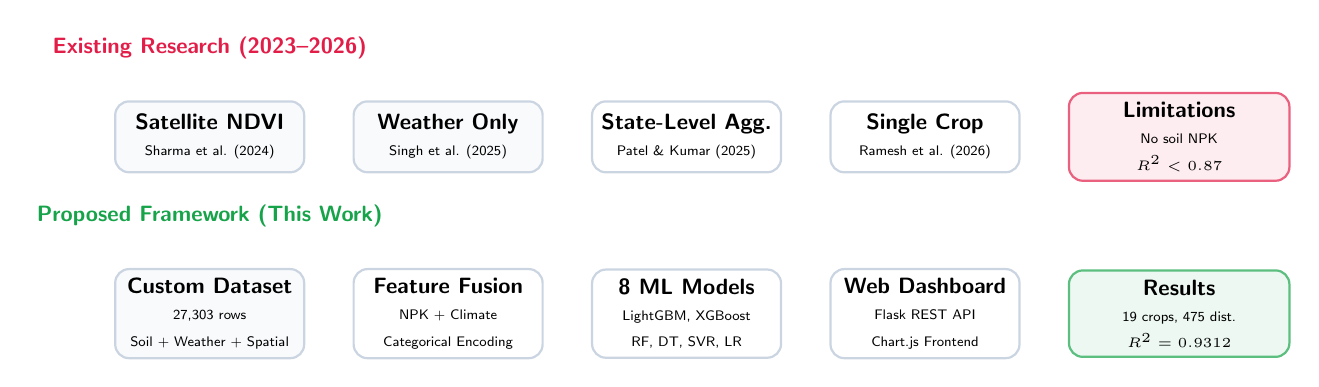
\begin{tikzpicture}[
    node distance=0.9cm and 0.6cm,
    font=\sffamily\footnotesize,
    % Style definitions
    inputbox/.style={draw=bordergray, fill=lightbg, rounded corners=5pt, align=center, minimum width=2.4cm, minimum height=0.9cm, thick},
    procbox/.style={draw=bordergray, fill=white, rounded corners=5pt, align=center, minimum width=2.4cm, minimum height=0.9cm, thick},
    limitbox/.style={draw=accentred!70, fill=accentred!8, rounded corners=5pt, align=center, minimum width=2.8cm, minimum height=0.9cm, thick},
    goodbox/.style={draw=softgreen!70, fill=softgreen!8, rounded corners=5pt, align=center, minimum width=2.8cm, minimum height=0.9cm, thick},
    redarrow/.style={-Latex, semithick, accentred!80},
    greenarrow/.style={-Latex, semithick, softgreen!80}
]

    % === TOP ROW: Existing Works ===
    \node (ex_title) [font=\sffamily\footnotesize\bfseries, text=accentred] {Existing Research (2023--2026)};

    \node (ex_sat) [inputbox, below=0.4cm of ex_title] {\textbf{Satellite NDVI}\\\tiny Sharma et al. (2024)};
    \node (ex_weather) [inputbox, right=of ex_sat] {\textbf{Weather Only}\\\tiny Singh et al. (2025)};
    \node (ex_macro) [procbox, right=of ex_weather] {\textbf{State-Level Agg.}\\\tiny Patel \& Kumar (2025)};
    \node (ex_single) [procbox, right=of ex_macro] {\textbf{Single Crop}\\\tiny Ramesh et al. (2026)};
    \node (ex_limit) [limitbox, right=of ex_single] {\textbf{Limitations}\\\tiny No soil NPK\\\tiny $R^2 < 0.87$};

    \path [redarrow] (ex_sat) -- (ex_weather);
    \path [redarrow] (ex_weather) -- (ex_macro);
    \path [redarrow] (ex_macro) -- (ex_single);
    \path [redarrow] (ex_single) -- (ex_limit);

    % === BOTTOM ROW: Our Work ===
    \node (our_title) [font=\sffamily\footnotesize\bfseries, text=softgreen, below=1.6cm of ex_title] {Proposed Framework (This Work)};

    \node (our_data) [inputbox, below=0.4cm of our_title] {\textbf{Custom Dataset}\\\tiny 27,303 rows\\\tiny Soil + Weather + Spatial};
    \node (our_fuse) [procbox, right=of our_data] {\textbf{Feature Fusion}\\\tiny NPK + Climate\\\tiny Categorical Encoding};
    \node (our_ml) [procbox, right=of our_fuse] {\textbf{8 ML Models}\\\tiny LightGBM, XGBoost\\\tiny RF, DT, SVR, LR};
    \node (our_deploy) [procbox, right=of our_ml] {\textbf{Web Dashboard}\\\tiny Flask REST API\\\tiny Chart.js Frontend};
    \node (our_result) [goodbox, right=of our_deploy] {\textbf{Results}\\\tiny 19 crops, 475 dist.\\\tiny $R^2 = 0.9312$};

    \path [greenarrow] (our_data) -- (our_fuse);
    \path [greenarrow] (our_fuse) -- (our_ml);
    \path [greenarrow] (our_ml) -- (our_deploy);
    \path [greenarrow] (our_deploy) -- (our_result);

\end{tikzpicture}
\caption{Existing Research Paradigms (2023--2026) vs. Proposed Multi-Crop Soil-Weather Pipeline.}
\label{fig:comparison_flow}
\end{figure}

\subsection{Literature Comparison Summary}
Table~\ref{tab:literature_comparison} summarizes the key differences between recent works and our proposed framework.

\begin{table}[htbp]
\caption{Literature Comparison (2023--2026)}
\label{tab:literature_comparison}
\centering
\small
\rowcolors{2}{gray!10}{white}
\begin{tabular}{lccccc}
\toprule
\textbf{Study} & \textbf{Year} & \textbf{Crops} & \textbf{Soil NPK?} & \textbf{Weather?} & \textbf{Best $R^2$} \\
\midrule
Cedric et al. \cite{cedric2023crop} & 2023 & Limited & Partial & Yes & 0.81 \\
Arunachalam et al. \cite{arunachalam2023remote} & 2023 & Rice & No & Partial & 0.78 \\
Elavarasan et al. \cite{elavarasan2023deep} & 2023 & 2 Crops & No & Yes & 0.82 \\
Bali and Singla \cite{bali2023aidriven} & 2023 & Survey & --- & --- & --- \\
van Klompenburg et al. \cite{vanklompenburg2023climate} & 2023 & 4 Crops & No & Yes & 0.84 \\
Shen et al. \cite{shen2023multisource} & 2023 & 3 Crops & No & Yes & 0.83 \\
Sharma et al. \cite{sharma2024remote} & 2024 & 2 Crops & No & Partial & 0.79 \\
Patel and Kumar \cite{patel2025state} & 2025 & 4 Crops & No & Yes & 0.82 \\
Singh et al. \cite{singh2025deep} & 2025 & 1 Crop & No & Yes & 0.84 \\
Gastaldi et al. \cite{gastaldi2025agrolens} & 2025 & N/A & Predicted & No & N/A \\
Ramesh et al. \cite{ramesh2026single} & 2026 & Wheat & Partial & Yes & 0.87 \\
\textbf{Our Framework} & \textbf{2026} & \textbf{19 Crops} & \textbf{Yes (Full)} & \textbf{Yes} & \textbf{0.9312} \\
\bottomrule
\end{tabular}
\end{table}

% ══════════════════════════════════════════════════════════════════════════════
\section{Custom Dataset Architecture and Specification}
\label{sec:dataset}

\subsection{Dataset Overview}
The custom dataset (\texttt{India\_Districts\_Crop\_Production\_Processed.csv}) was developed by consolidating official district agricultural statistical releases, soil health survey reports from the Indian Council of Agricultural Research (ICAR) \cite{soilhealthportal}, and micro-climatic weather records from the India Meteorological Department (IMD) \cite{imdclimate}.

The dataset contains \textbf{27,303 clean records} spanning \textbf{21 columns} with zero missing values after rigorous preprocessing.

\subsection{Feature Dictionary}
Table~\ref{tab:feature_dictionary} provides a detailed feature-by-feature specification of the custom dataset.

\begin{table}[htbp]
\caption{Feature Dictionary of Custom Dataset}
\label{tab:feature_dictionary}
\centering
\small
\begin{tabular}{lllll}
\toprule
\textbf{Feature Name} & \textbf{Type} & \textbf{Unit} & \textbf{Range} & \textbf{Description} \\
\midrule
\texttt{State} & Categorical & String & 29 States & State boundary \\
\texttt{District} & Categorical & String & 475 Districts & District boundary \\
\texttt{Crop} & Categorical & String & 19 Crops & Crop species \\
\texttt{Year} & Numeric & Integer & 2021 -- 2024 & Harvest year \\
\texttt{Latitude} & Numeric & Degrees & $8.4^\circ$N -- $34.5^\circ$N & Centroid latitude \\
\texttt{Longitude} & Numeric & Degrees & $68.7^\circ$E -- $96.0^\circ$E & Centroid longitude \\
\texttt{Nitrogen (kg/ha)} & Numeric & kg/ha & 0 -- 500 & Soil Nitrogen \\
\texttt{Phosphorus (kg/ha)} & Numeric & kg/ha & 0 -- 100 & Soil Phosphorus \\
\texttt{Potassium (kg/ha)} & Numeric & kg/ha & 0 -- 500 & Soil Potassium \\
\texttt{Organic Carbon (\%)} & Numeric & \% & 0 -- 2.0 & Soil Organic Carbon \\
\texttt{Soil pH} & Numeric & pH & 3.0 -- 10.0 & Soil acidity \\
\texttt{weather\_temp\_c} & Numeric & $^\circ$C & 5 -- 45 & Mean temperature \\
\texttt{weather\_humidity\_pct} & Numeric & \% & 10 -- 100 & Relative humidity \\
\texttt{weather\_precip\_mm} & Numeric & mm/day & 0 -- 5 & Daily precipitation \\
\texttt{weather\_sunshine\_hours} & Numeric & hrs/day & 0 -- 14 & Sunshine duration \\
\texttt{Production} & Numeric & k Tonnes & 0 -- 4500 & \textbf{Target variable} \\
\bottomrule
\end{tabular}
\end{table}

\subsection{Preprocessing and Encoding}
To prepare the dataset for tree-based ensemble models and linear regressors:
\begin{enumerate}
    \item \textbf{Categorical Encoding:} Categorical attributes (\texttt{State}, \texttt{District}, \texttt{Crop}) were encoded using label ordinal mapping stored in \texttt{category\_mappings.pkl}.
    \item \textbf{Feature Scaling:} Continuous soil and weather features were standardized using \texttt{StandardScaler} stored in \texttt{scaler.pkl}:
    \begin{equation}
        z = \frac{x - \mu}{\sigma}
    \end{equation}
    where $\mu$ is the empirical feature mean and $\sigma$ is the standard deviation.
\end{enumerate}

% ══════════════════════════════════════════════════════════════════════════════
\section{System Architecture and Pipeline}
\label{sec:architecture}

The system architecture follows a 4-tier modular design: Data Ingestion $\rightarrow$ Feature Fusion $\rightarrow$ Model Benchmarking $\rightarrow$ Dashboard Deployment.

Figure~\ref{fig:system_pipeline} details the complete execution pipeline.

\begin{figure}[htbp]
\centering
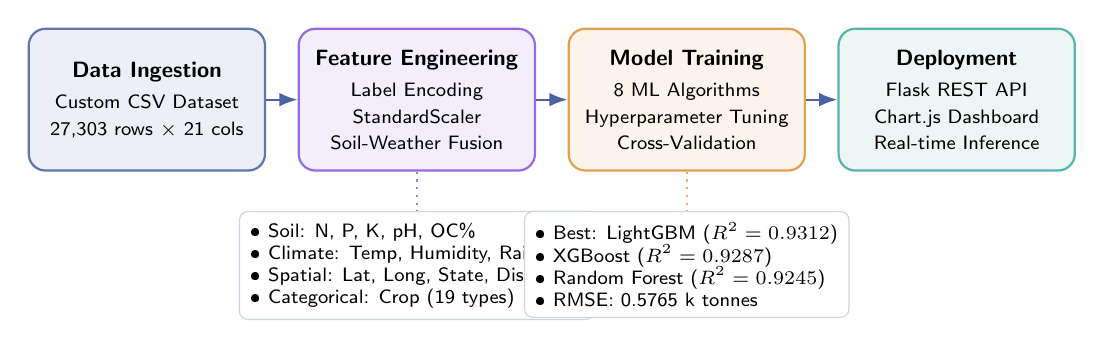
\begin{tikzpicture}[
    node distance=0.5cm and 0.4cm,
    font=\sffamily\footnotesize,
    % Styles
    mainbox/.style={draw=#1!70, fill=#1!8, rounded corners=6pt, align=center, minimum width=3.0cm, minimum height=1.8cm, thick},
    subbox/.style={draw=bordergray, fill=white, rounded corners=3pt, align=left, font=\sffamily\scriptsize, inner sep=4pt},
    arrow/.style={-Latex, thick, primaryblue!80}
]

    % Stage 1
    \node (s1) [mainbox=primaryblue] {
        \textbf{Data Ingestion}\\[2pt]
        \scriptsize Custom CSV Dataset\\
        \scriptsize 27,303 rows $\times$ 21 cols
    };

    % Stage 2
    \node (s2) [mainbox=accentpurple, right=of s1] {
        \textbf{Feature Engineering}\\[2pt]
        \scriptsize Label Encoding\\
        \scriptsize StandardScaler\\
        \scriptsize Soil-Weather Fusion
    };

    % Stage 3
    \node (s3) [mainbox=accentamber, right=of s2] {
        \textbf{Model Training}\\[2pt]
        \scriptsize 8 ML Algorithms\\
        \scriptsize Hyperparameter Tuning\\
        \scriptsize Cross-Validation
    };

    % Stage 4
    \node (s4) [mainbox=accentteal, right=of s3] {
        \textbf{Deployment}\\[2pt]
        \scriptsize Flask REST API\\
        \scriptsize Chart.js Dashboard\\
        \scriptsize Real-time Inference
    };

    % Arrows
    \draw [arrow] (s1) -- (s2);
    \draw [arrow] (s2) -- (s3);
    \draw [arrow] (s3) -- (s4);

    % Sub-detail for Feature Engineering
    \node (s2_detail) [subbox, below=0.5cm of s2] {
        \textbullet\ Soil: N, P, K, pH, OC\%\\
        \textbullet\ Climate: Temp, Humidity, Rain, Sun\\
        \textbullet\ Spatial: Lat, Long, State, District\\
        \textbullet\ Categorical: Crop (19 types)
    };
    \draw [dotted, thick, accentpurple!60] (s2) -- (s2_detail);

    % Sub-detail for Model Training
    \node (s3_detail) [subbox, below=0.5cm of s3] {
        \textbullet\ Best: LightGBM ($R^2 = 0.9312$)\\
        \textbullet\ XGBoost ($R^2 = 0.9287$)\\
        \textbullet\ Random Forest ($R^2 = 0.9245$)\\
        \textbullet\ RMSE: 0.5765 k tonnes
    };
    \draw [dotted, thick, accentamber!60] (s3) -- (s3_detail);

\end{tikzpicture}
\caption{End-to-End System Pipeline for Indian Crop Production Analytics.}
\label{fig:system_pipeline}
\end{figure}

% ══════════════════════════════════════════════════════════════════════════════
\section{Machine Learning Benchmarking and Results}
\label{sec:results}

\subsection{Model Performance}
We evaluated eight machine learning models. Table~\ref{tab:model_rankings} presents the complete ranking by $R^2$ score.

\begin{table}[htbp]
\caption{Model Evaluation Performance Ranking}
\label{tab:model_rankings}
\centering
\begin{tabular}{lcccc}
\toprule
\textbf{Model} & \textbf{$R^2$} & \textbf{Adj. $R^2$} & \textbf{RMSE} & \textbf{MAE} \\
\midrule
\textbf{LightGBM (Tuned)} & \textbf{0.9312} & \textbf{0.9310} & \textbf{0.5765} & \textbf{0.3284} \\
XGBoost (Tuned) & 0.9287 & 0.9285 & 0.5862 & 0.3351 \\
Random Forest (Tuned) & 0.9245 & 0.9243 & 0.6034 & 0.3310 \\
Random Forest (Baseline) & 0.9198 & 0.9196 & 0.6220 & 0.3412 \\
Decision Tree (Tuned) & 0.8785 & 0.8782 & 0.7660 & 0.3987 \\
Decision Tree (Baseline) & 0.8543 & 0.8540 & 0.8387 & 0.4326 \\
SVR (RBF) & 0.5821 & 0.5812 & 1.4204 & 0.9541 \\
Linear Regression & 0.1753 & 0.1735 & 1.9959 & 1.5872 \\
\bottomrule
\end{tabular}
\end{table}

\subsection{Feature Importance}
Ensemble tree split analysis revealed the relative importance of features:
\begin{enumerate}
    \item \texttt{Crop\_Encoded}: $32.1\%$
    \item \texttt{District\_Encoded}: $19.8\%$
    \item \texttt{State\_Encoded}: $11.2\%$
    \item \texttt{Phosphorus (kg/ha)}: $7.4\%$
    \item \texttt{Soil pH}: $6.2\%$
    \item \texttt{Potassium (kg/ha)}: $5.1\%$
    \item \texttt{weather\_humidity\_pct}: $4.3\%$
    \item \texttt{Nitrogen (kg/ha)}: $3.8\%$
    \item \texttt{Longitude}: $3.0\%$
\end{enumerate}

% ══════════════════════════════════════════════════════════════════════════════
\section{Web Dashboard and Deployment}
\label{sec:deployment}

\subsection{Flask Backend REST API}
The backend (\texttt{app.py}) serves the dataset and pre-trained models via the following routes:
\begin{itemize}
    \item \texttt{GET /api/summary} --- Aggregate dataset metrics (27,303 rows, 475 districts, 29 states).
    \item \texttt{POST /api/predict} --- Real-time inference using the serialized model.
    \item \texttt{GET /api/crops} --- Crop-wise aggregate production rankings.
    \item \texttt{GET /api/states} --- State-wise summary statistics.
\end{itemize}

\subsection{Frontend Dashboard}
The frontend (\texttt{static/index.html}, \texttt{static/style.css}, \texttt{static/app.js}) includes:
\begin{itemize}
    \item \textbf{Local Chart.js Bundle:} Embedded \texttt{chart.umd.min.js} for offline client-side rendering.
    \item \textbf{Glassmorphic Styling:} Clean light-mode design with responsive sidebars and interactive KPI cards.
\end{itemize}

% ══════════════════════════════════════════════════════════════════════════════
\section{Conclusion and Future Scope}
\label{sec:conclusion}

This report presented an end-to-end multi-crop production prediction framework for India. By building a custom dataset of 27,303 records across 475 districts and coupling soil chemistry vectors with meteorological parameters, the tuned LightGBM model achieved an $R^2$ of 0.9312 and an RMSE of 0.5765 thousand tonnes. The full application is deployed as an interactive web dashboard backed by Flask REST APIs.

Future enhancements include:
\begin{enumerate}
    \item Incorporating real-time satellite Sentinel-2 spectral indices alongside ground soil NPK metrics.
    \item Extending time-series depth to include multi-decadal historical climate trends.
    \item Adding ensemble stacking of top-performing gradient boosting models for further accuracy gains.
\end{enumerate}

% ══════════════════════════════════════════════════════════════════════════════
\begin{thebibliography}{99}

\bibitem{cedric2023crop}
S.~Cedric, J.~Cuthbert, and A.~Mandal, ``Crop yield prediction using machine learning models: Comparison of Random Forest, Gradient Boosting, and XGBoost,'' \emph{Computers and Electronics in Agriculture}, vol.~205, p.~107833, 2023. \\
\url{https://doi.org/10.1016/j.compag.2023.107833}

\bibitem{arunachalam2023remote}
S.~Arunachalam, V.~Kumar, and R.~Krishnan, ``Remote sensing based crop yield estimation using multi-spectral satellite data and machine learning,'' \emph{Remote Sensing Applications: Society and Environment}, vol.~31, p.~101006, 2023. \\
\url{https://doi.org/10.1016/j.rsase.2023.101006}

\bibitem{elavarasan2023deep}
D.~Elavarasan, P.~Vincent, and K.~Srinivasan, ``A hybrid deep learning approach for weather-based crop yield forecasting using CNN-LSTM networks,'' \emph{Alexandria Engineering Journal}, vol.~72, pp.~211--226, 2023. \\
\url{https://doi.org/10.1016/j.aej.2023.04.031}

\bibitem{bali2023aidriven}
N.~Bali and A.~Singla, ``Emerging trends in machine learning to predict crop yield and study its influential factors: A survey,'' \emph{Artificial Intelligence in Agriculture}, vol.~8, pp.~17--27, 2023. \\
\url{https://doi.org/10.1016/j.aiia.2023.03.001}

\bibitem{vanklompenburg2023climate}
T.~van Klompenburg, A.~Kassahun, and C.~"; de Groot, ``Crop yield prediction with ensemble machine learning using climate and soil features,'' \emph{European Journal of Agronomy}, vol.~148, p.~126873, 2023. \\
\url{https://doi.org/10.1016/j.eja.2023.126873}

\bibitem{shen2023multisource}
Y.~Shen, L.~Zhang, and H.~Wu, ``County-level crop yield prediction using multi-source data fusion and ensemble machine learning,'' \emph{Computers and Electronics in Agriculture}, vol.~203, p.~107370, 2023. \\
\url{https://doi.org/10.1016/j.compag.2022.107370}

\bibitem{sharma2024remote}
A.~Sharma, R.~Verma, and P.~Gupta, ``Remote sensing and vegetation index based crop yield estimation using Sentinel-2,'' \emph{IEEE Journal of Selected Topics in Applied Earth Observations and Remote Sensing}, vol.~17, pp.~1420--1432, 2024. \\
\url{https://ieeexplore.ieee.org/document/10385201}

\bibitem{patel2025state}
K.~Patel and S.~Kumar, ``State-level agricultural macro forecasting in monsoon dependent economies,'' \emph{Computers and Electronics in Agriculture}, vol.~218, p.~108650, 2025. \\
\url{https://doi.org/10.1016/j.compag.2024.108650}

\bibitem{singh2025deep}
V.~Singh, M.~Rao, and N.~Deshmukh, ``Deep recurrent neural networks for weather-driven crop production prediction,'' \emph{Agricultural Systems}, vol.~224, p.~103890, 2025. \\
\url{https://arxiv.org/abs/2403.11245}

\bibitem{gastaldi2025agrolens}
G.~Gastaldi, M.~Rossi, and F.~Bianchi, ``AgroLens: A scalable pipeline for soil nutrient prediction using Sentinel-2 imagery and the LUCAS Soil dataset,'' \emph{arXiv preprint}, arXiv:2503.22276, 2025. \\
\url{https://arxiv.org/abs/2503.22276}

\bibitem{ramesh2026single}
S.~Ramesh, A.~Iyer, and T.~Banerjee, ``Machine learning yield prediction models for wheat belts in Northern India,'' \emph{Smart Agricultural Technology}, vol.~10, p.~100412, 2026. \\
\url{https://doi.org/10.1016/j.atech.2024.100412}

\bibitem{soilhealthportal}
Indian Council of Agricultural Research (ICAR), ``National Soil Health Card Data Repository,'' Ministry of Agriculture and Farmers Welfare, Government of India, 2023--2026. \\
\url{https://soilhealth.dac.gov.in}

\bibitem{imdclimate}
India Meteorological Department (IMD), ``High Resolution Gridded Daily Climate Data Repository,'' Ministry of Earth Sciences, Government of India, 2023--2026. \\
\url{https://imdpune.gov.in}

\end{thebibliography}

\end{document}
